\subsection{Applications of Complex Analysis}

\subsubsection{Real Integrals}
\textit{Type I:}\\
If we have an integral of the form
\[\int_0^{2\pi} F(\cos\theta,\sin\theta)d\theta\]
then we can use the substitution $z=e^{i\theta}$ to convert this into a contour integral around the unit circle. We can then use the residue theorem to evaluate the integral.
\begin{align*}
    &\to\oint_{|z|=1} F\brround{\frac{z+z^{-1}}{2},\frac{z-z^{-1}}{2i}}\frac{dz}{iz}=\oint_{|z|=1} f(z)dz=2\pi i\sum_{j=1}^N\Res(f(z);z_j)
\end{align*}
Ex:
\begin{align*}
    &\int_0^\pi\frac{d\theta}{1+\sin^2\theta}\\
    &f(z)=f(-z)\Ra I=\frac{1}{2}\int_0^{2\pi}\frac{d\theta}{1+\sin^2\theta}\\
    &z=e^{i\theta}\Ra dz=ie^{i\theta}d\theta\Ra \frac{dz}{iz}=d\theta\\
    &\sin^2\theta=\frac{1}{(2i)^2}\brround{z-z^{-1}}^2=-\frac{1}{4}\brround{z^2-2+z^{-2}}\\
    &I=\frac{1}{2i}\int_{|z|=1}\frac{dz}{z(1-\frac{1}{4}(z^2-2+z^{-2}))}=-2i\int_{|z|=1}\frac{zdz}{z^2(4-z^2+2-z^{-2})}=2i\int_{|z|=1}\frac{zdz}{z^4-6z^2+1}\\
    &z^2=\frac{6\pm\sqrt{36-4}}{2}=3\pm2\sqrt{2}\Ra z_{1,2}=\pm\sqrt{3-2\sqrt{2}}\\
    &I=2i\int_{|z|=1}\frac{zdz}{(z^2-z_{1,2}^2)(z^2-z_{3,4}^2)}\\
    &Q'(z)=4z^3-12z\\
    &\frac{P(z)}{Q'(z)}=\frac{1}{4(z^2-3)}\\
    &I=2(2i)(2\pi i)\frac{1}{4((3-2\sqrt{2})-3)}=\frac{\pi}{\sqrt{2}}
\end{align*}
Ex2:
\begin{align*}
    &\int_0^{2\pi}\frac{\sin^2\theta}{3+\cos\theta}d\theta\\
    &z=e^{i\theta}\Ra dz=ie^{i\theta}d\theta\Ra d\theta=\frac{dz}{iz}\\
    &\sin^2\theta=-\frac{1}{4}\brround{z-z^{-1}}=-\frac{1}{4}\brround{z^2-2+z^{-2}}\\
    &\cos\theta=\frac{1}{2}\brround{z+z^{-1}}\\
    &I=-\frac{1}{i}\int_{|z|=1}\frac{\frac{1}{4}\brround{z^2-2+z^{-2}}dz}{z(3+\frac{1}{2}(z+z^{-1}))}=-\frac{1}{2i}\int_{|z|=1}\frac{z^4-2z^2+1}{z^3(6+z+z^{-1})}dz=-\frac{1}{2i}\int_{|z|=1}\frac{z^4-2z^2+1}{z^2(z^2+6z+1)}dz\\
    &z_1=0,\ z_{2,3}=-3\pm2\sqrt{2}\Ra z_2=2\sqrt{2}-3\\
    &f_1(z)=\frac{z^4-2z^2+1}{z^2+6z+1}\Ra f_1'(z)=\frac{(z^2+6z+1)(4z^3-4z)-(z^4-2z^2+1)(2z+6)}{(z^2+6z+1)^2}\\
    &\Res(f(z);0)=-\frac{1}{2i}f_1'(0)=\frac{3}{i}\\
    &Q(z)=z^4+6z^3+z^2\Ra Q'(z)=4z^3+18z^2+2z\\
    &\frac{P(z)}{Q(z)}=\frac{z^4-2z^2+1}{2z(2z^2+9z+1)}\\
    &-2i\Res(f(z);z_2)=\frac{z_2^4-2z_2^2+1}{2z_2(z_2^2+3z_2+z_2^2+6z_2+1)}=\frac{(z_2^2-1)^2}{2z_2^2(z_2+3)}=\frac{((2\sqrt{2}-3)^2-1)^2}{2(2\sqrt{2}-3)^2(2\sqrt{2})}\\
    &=\frac{(16-12\sqrt{2})^2}{4\sqrt{2}(8-12\sqrt{2}+9)}=\frac{4(4-3\sqrt{2})^2}{17\sqrt{2}-24}=\frac{4(16-24\sqrt{2}+18)}{17\sqrt{2}-24}=\frac{4(34-24\sqrt{2})}{17\sqrt{2}-24}=\frac{4\sqrt{2}(34-24\sqrt{2})}{34-24\sqrt{2}}\\
    &=4\sqrt{2}\\
    &\Res(f(z);z_2)=-\frac{2\sqrt{2}}{i}\\
    &I=2\pi i\brround{\frac{3}{i}-\frac{2\sqrt{2}}{i}}=2\pi(3-2\sqrt{2})
\end{align*}
\textit{Type II:}\\
If we have an integral of the form
\[\int_{-\infty}^\infty\frac{P(x)}{Q(x)}dx\]
where $P(x)$ and $Q(x)$ are polynomials and $\deg Q(x)\geq\deg P(x)+2$, then we can use the half-moon contour and solve for the part of the contour that runs along the real axis.\\
\centerline{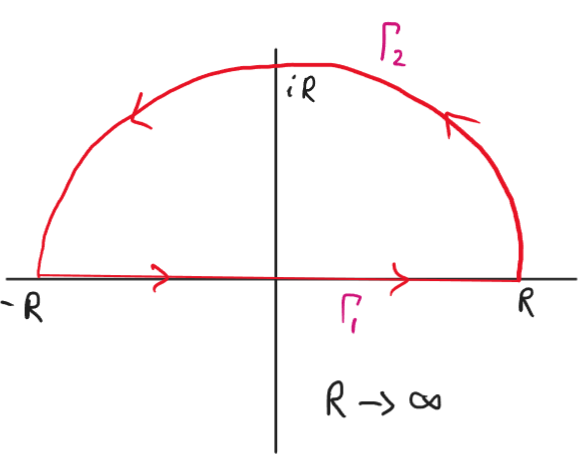
\includegraphics[width=0.6\textwidth]{Images/ComplexAnalysisPictures/HalfMoon.png}}
\begin{align*}
    &\int_{-\infty}^\infty\frac{x^2+2x+2}{x^4+x^2+1}dx\\
    &\deg(Q)\geq\deg(P)+2\Ra I=\int\frac{z^2+2z+2}{z^4+z^2+1}\\
    &z^2=\frac{-1\pm\sqrt{1-4}}{2}=-\frac{1}{2}\pm\frac{\sqrt{3}}{2}i=e^{\pm i\frac{2\pi}{3}}\\
    &z=\brcurly{e^{\pm i\frac{\pi}{3}},e^{\pm i\frac{2\pi}{3}}}\\
    &Q'(z)=4z^3+2z\\
    &\frac{P(z)}{Q'(z)}=\frac{z^2+2z+2}{4z^3+2z}\\
    &\Res(f(z);e^{i\frac{\pi}{3}})=\frac{e^{i\frac{2\pi}{3}}+2e^{i\frac{\pi}{3}}+2}{2(2e^{i\pi}+e^{i\frac{\pi}{3}})}=\frac{-\frac{1}{2}+i\frac{\sqrt{3}}{2}+1+i\sqrt{3}+2}{2(-2+\frac{1}{2}+i\frac{\sqrt{3}}{2})}=\frac{\frac{5}{2}+i\frac{3\sqrt{3}}{2}}{2(-\frac{3}{2}+i\frac{\sqrt{3}}{2})}=\frac{5+i3\sqrt{3}}{2(-3+i\sqrt{3})}\\
    &=\frac{(5+i3\sqrt{3})(-3-i\sqrt{3})}{24}=\frac{-15-i5\sqrt{3}-i9\sqrt{3}+9}{24}=\frac{-6-i14\sqrt{3}}{24}\\
    &\Res(f(z);e^{i\frac{2\pi}{3}})=\frac{e^{i\frac{4\pi}{3}}+2e^{i\frac{2\pi}{3}}+2}{2(2e^{i2\pi}+e^{i\frac{2\pi}{3}})}=\frac{-\frac{1}{2}-i\frac{\sqrt{3}}{2}-1+i\sqrt{3}+2}{2(2-\frac{1}{2}+i\frac{\sqrt{3}}{2})}=\frac{\frac{1}{2}+i\frac{\sqrt{3}}{2}}{2(\frac{3}{2}+i\frac{\sqrt{3}}{2})}=\frac{1+i\sqrt{3}}{2(3+i\sqrt{3})}\\
    &=\frac{(1+i\sqrt{3})(3-i\sqrt{3})}{24}=\frac{3-i\sqrt{3}+i3\sqrt{3}+3}{24}=\frac{6+i2\sqrt{3}}{24}\\
    &I=2\pi i\brround{\Res(f(z);e^{i\frac{\pi}{3}}+\Res(f(z);e^{i\frac{2\pi}{3}})}=\frac{\pi i}{12}\brround{-6-i14\sqrt{3}+6+i2\sqrt{3}}=\frac{\pi i}{12}\brround{-i12\sqrt{3}}\\
    &I=\pi\sqrt{3}
\end{align*}
Ex2:
\begin{align*}
    &\int_0^\infty\frac{x^2}{(x^2+4)^2}dx\\
    &f(x)=f(-x)\\
    &I=\frac{1}{2}\int_{-\infty}^\infty\frac{x^2}{(x^2+4)^2}dx\\
    &\deg(Q)\geq\deg(P)+2\Ra I=\frac{1}{2}\int\frac{z^2}{(z^2+4)^2}dz\\
    &z=\pm 2i\Ra z_1=2i\\
    &f(z)=\frac{z^2}{(z+2i)^2(z-2i)^2}\Ra f_1(z)=\frac{z^2}{(z+2i)^2}\\
    &f_1'(z)=\frac{2z}{z+2i}\brround{\frac{1}{z+2i}-\frac{z}{(z+2i)^2}}\\
    &f_1'(i)=\frac{4i}{4i}\brround{\frac{1}{4i}-\frac{2i}{-16}}=-\frac{i}{4}+\frac{i}{8}=-\frac{i}{8}=\Res(f(z);i)\\
    &I=\frac{1}{2}2\pi i\brround{-\frac{i}{8}}=\frac{\pi}{8}
\end{align*}
\textit{Type III:}\\
If we have an integral of the form
\[\int_0^\infty\frac{dx}{1+x^n}\]
we can expose the symmetry of the problem and use the pizza contour to solve the integral.\\
\centerline{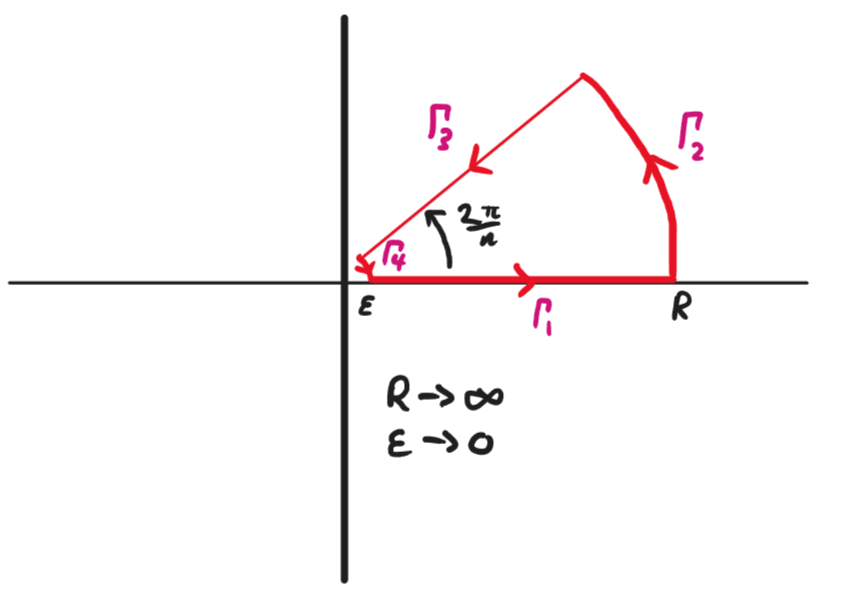
\includegraphics[width=0.6\textwidth]{Images/ComplexAnalysisPictures/Pizza.png}}
\begin{align*}
    &\int_0^\infty\frac{dx}{x^3+1}\\
    &z^3+1=0\\
    &z^3=-e^{2k\pi i}=e^{\pi i+2k\pi i}\\
    &z=e^{i\frac{\pi}{3}+i\frac{2k\pi}{3}}=\frac{1}{2}+i\frac{\sqrt{3}}{2}\\
    &\int_0^R\frac{dz}{z^3+1}+\int_{C_R}\frac{dz}{z^3+1}+\int_{\Gamma}\frac{dz}{z^3+1}=2\pi i\Res(f(z);\tfrac{1}{2}+i\tfrac{\sqrt{3}}{2})\\
    &Q'(z)=3z^2\\
    &\frac{P(z)}{Q'(z)}=\frac{1}{3z^2}=\frac{1}{3e^{i\frac{2\pi i}{3}}}=\frac{1}{6}\brround{-1-i\sqrt{3}}=\Res(f(z);e^{i\frac{\pi}{3}})\\
    &\int_{C_R}\frac{dz}{z^3+1}\Ra \brvertical{\int_{C_R}\frac{dz}{z^3+1}}\leq\max_{|z|=R}\brvertical{\frac{1}{R^3+1}}\frac{\pi R}{3}\to0\\
    &\int_{\Gamma}\frac{dz}{z^3+1}=-\int_0^R\frac{e^{i\frac{2\pi}{3}}dz}{z^3+1}\\
    &\int_0^R\frac{dz}{z^3+1}-\int_0^R\frac{e^{\frac{2\pi i}{3}}dz}{z^3+1}\\
    &I\brround{1-e^{i\frac{2\pi}{3}}}=\frac{1}{3}e^{-i\frac{2\pi}{3}}\\
    &I\brround{e^{-i\frac{\pi}{3}}-e^{i\frac{\pi}{3}}}=-2i\sin\bfrac{\pi}{3}I=2\pi i\frac{1}{3}e^{-i\pi}\\
    &I=\frac{\pi}{3\sin\bfrac{\pi}{3}}=\frac{2\pi}{3\sqrt{3}}
\end{align*}
\textit{Type IV:}\\
If we have an integral of the form
\[\int_{-\infty}^\infty\frac{P(x)}{Q(x)}\sin(\beta x)dx\]
or
\[\int_{-\infty}^\infty\frac{P(x)}{Q(x)}\cos(\beta x)dx\]
where $P(x)$ and $Q(x)$ are polynomials and $\deg Q(x)\geq\deg P(x)+1$ and we use a similar method to before with the half-moon contour.\\
\centerline{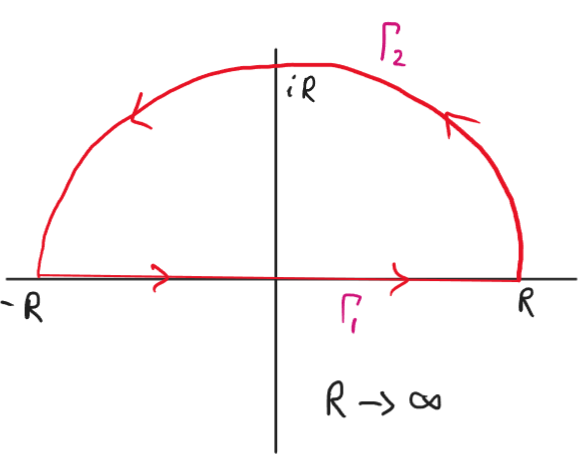
\includegraphics[width=0.6\textwidth]{Images/ComplexAnalysisPictures/HalfMoon.png}}
Ex:
\begin{align*}
    &\int_{-\infty}^\infty\frac{\sin x}{x^2+2x+2}dx\\
    &f(z)=\frac{e^{iz}}{z^2+2z+2}dz\\
    &z=\frac{-2\pm\sqrt{4-8}}{2}=-1\pm i\\
    &\int_{\Gamma_1}\frac{e^{iz}}{z^2+2z+2}dz+\int_{\Gamma_2}\frac{e^{iz}}{z^2+2z+2}dz=2\pi i\Res\brround{\frac{e^{iz}}{z^2+2z+2};-1+i}\\
    &\brvertical{\int_{\Gamma_1}\frac{e^{iz}}{z^2+2z+2}dz}\leq\max_{|z|=R}\brvertical{\frac{e^{iz}}{z^2+2z+2}}\pi R\leq\max_{0\leq t\leq \pi}\frac{\pi Re^{-R\sin t}}{R^2-2R-2}=\frac{\pi R}{R^2-2R-2}\to 0\\
    &Q(z)=z^2+2z+2\Ra Q'(z)=2(z+1)\\
    &Q'(-1+ i)=2i\\
    &\Res\brround{\frac{e^{iz}}{z^2+2z+2};-1+ i}=\frac{e^{-1-i}}{2i}\\
    &\int_{\Gamma_1}\frac{e^{iz}}{z^2+2z+2}dz=2\pi i\frac{e^{-1-i}}{2i}=\pi e^{-1}e^{-i}\\
    &\int_{-\infty}^\infty\frac{\sin x}{x^2+2x+2}dx=\Im\brround{\frac{\pi}{e}e^{-i}}=-\frac{\pi}{e}\sin(1)\\
    &\int_{-\infty}^\infty\frac{\cos x}{x^2+2x+2}dx=\Re\brround{\frac{\pi}{e}e^{-i}}=\frac{\pi}{e}\cos(1)
\end{align*}
Ex2:
\begin{align*}
    &\int_{-\infty}^\infty\frac{x\cos(2x)}{x^2+2x+5}dx\\
    &f(z)=\frac{ze^{i2z}}{z^2+2z+5}dz\\
    &z=\frac{-2\pm\sqrt{4-20}}{2}=-1\pm 2i\\
    &\int_{\Gamma_1}\frac{ze^{i2z}}{z^2+2z+5}dz+\int_{\Gamma_2}\frac{ze^{i2z}}{z^2+2z+5}dz=2\pi i\Res\brround{\frac{ze^{i2z}}{z^2+2z+5};-1+2i}\\
    &\Gamma_2:\ z=Re^{it}\\
    &\brvertical{\int_{\Gamma_2}f(z)dz}\leq\int_{\Gamma_2}\brvertical{f(z)}dz=\int_{\Gamma_2}\brvertical{\frac{ze^{i2z}}{z^2+2z+5}}dz=\int_{\Gamma_2}\brvertical{\frac{z}{z^2+2z+5}}e^{-2R\sin t}dz\\
    &\brvertical{\frac{z}{z^2+2z+5}}\leq\frac{R}{R^2-2R-5}\\
    &\int_{\Gamma_2}\brvertical{\frac{z}{z^2+2z+5}}e^{-2R\sin t}dz\leq\frac{R}{R^2-2R-5}\int_{\Gamma_2}e^{-2R\sin t}dz\\
    &\brvertical{\int_{\Gamma_2}e^{-2R\sin t}dz}\leq\max_{0\leq t\leq \pi}e^{-2R\sin t}\\
    &0\leq t\leq \pi\Ra 0\leq \sin t\leq 1\Ra \max_{0\leq t\leq \pi}e^{-2R\sin t}=1\\
    &\frac{R}{R^2-2R-5}\int_{\Gamma_2}e^{-2R\sin t}dz\leq\frac{R}{R^2-2R-5}\to 0\\
    &\Ra \int_{\Gamma_2}f(z)dz\to0\\
    &Q(z)=z^2+2z+5\Ra Q'(z)=2(z+1)\\
    &Q'(-1+2i)=4i\\
    &\Res\brround{\frac{ze^{i2z}}{z^2+2z+5};-1+2i}=\frac{(-1+2i)e^{2i(-1+2i)}}{4i}=\frac{(-1+2i)}{4i}e^{-4-2i}\\
    &\int_{\Gamma_1}\frac{ze^{i2z}}{z^2+2z+5}dz=2\pi i\frac{(-1+2i)}{4i}e^{-4}(\cos(2)-i\sin(2))=\frac{\pi}{2e^4}\brround{-\cos(2)+2\sin(2)+i\sin(2)+2i\cos(2)}\\
    &I=\frac{\pi}{2e^4}(2\sin(2)-\cos(2))
\end{align*}
Note that if we have $\beta<0$ then we use the half-moon contour but flipped across the real axis.\\
\textit{Type V:}\\
If we have an integral of the form
\[\int_{-\infty}^\infty\frac{e^{\beta x}}{1+e^x}dx\]
with $0<\beta<1$\\
We can use the box contour to solve the integral.\\
\centerline{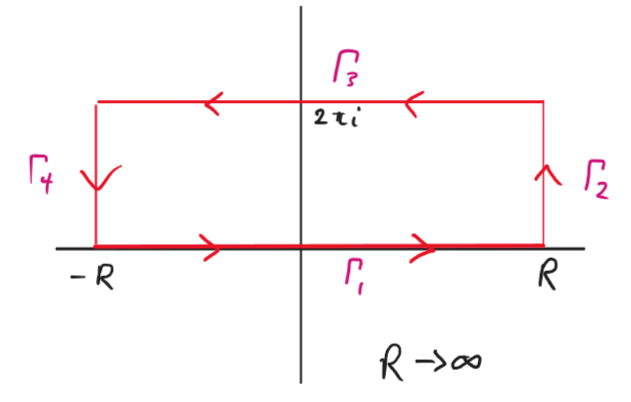
\includegraphics[width=0.6\textwidth]{Images/ComplexAnalysisPictures/Box.png}}
Ex:
\begin{align*}
    &\int_{-\infty}^\infty\frac{e^{\frac{x}{3}}}{(e^x+1)^2}dx\\
    &f(z)=\frac{e^{\frac{z}{3}}}{(e^z+1)^2}\\
    &I=\int_{\Gamma_1}\frac{e^{\frac{z}{3}}}{(e^z+1)^2}dz\\
    &e^z+1=e^x(\cos(y)+i\sin(y))+1=0\Ra z=\pi i(2n+1)\\
    &z_1=\pi i\\
    &w=z-\pi i\\
    &\frac{e^{\frac{z}{3}}}{(e^z+1)^2}=\frac{e^{\frac{w+\pi i}{3}}}{(e^{w+\pi i}+1)^2}=\frac{e^{i\frac{\pi}{3}}\brround{1+\frac{w}{3}+\bigO(w^2)}}{(-e^w+1)^2}=e^{i\frac{\pi}{3}}\brround{1+\frac{w}{3}+\bigO(w^2)}\brround{-w-\frac{w^2}{2}+\bigO(w^3)}^{-2}\\
    &=\frac{e^{i\frac{\pi}{3}}}{w^2}\brround{1+\frac{w}{3}+\bigO(w^2)}\brround{1+\frac{w}{2}+\bigO(w^2)}^{-2}=\frac{e^{i\frac{\pi}{3}}}{w^2}\brround{1+\frac{w}{3}+\bigO(w^2)}\brround{1-w+\bigO(w^2)}\\
    &=\frac{e^{i\frac{\pi}{3}}}{w^2}\brround{1-\frac{2w}{3}+\bigO(w^2)}\\
    &\Res\brround{\frac{e^{\frac{z}{3}}}{(e^z+1)^2};\pi i}=-\frac{2e^{i\frac{\pi}{3}}}{3}\\
    &\int_{\Gamma_1}\frac{e^{\frac{z}{3}}}{(e^z+1)^2}dz+\int_{\Gamma_2}\frac{e^{\frac{z}{3}}}{(e^z+1)^2}dz+\int_{\Gamma_3}\frac{e^{\frac{z}{3}}}{(e^z+1)^2}dz+\int_{\Gamma_4}\frac{e^{\frac{z}{3}}}{(e^z+1)^2}dz=2\pi i\Res\brround{\frac{e^{\frac{z}{3}}}{(e^z+1)^2};\pi i}\\
    &\Gamma_2,\ \Gamma_4:\ z=\pm R+iy,\ 0\leq y\leq 2\pi\\
    &\int_{\Gamma_2}\frac{e^{\frac{z}{3}}}{(e^z+1)^2}dz=-\int_{\Gamma_4}\frac{e^{\frac{z}{3}}}{(e^z+1)^2}dz\\
    &\int_{\Gamma_2}\frac{e^{\frac{z}{3}}}{(e^z+1)^2}dz=\int_0^{2\pi}\frac{e^{\frac{ R+iy}{3}}}{(e^{R+iy}+1)^2}dz\\
    &\brvertical{\int_{\Gamma_2}\frac{e^{\frac{z}{3}}}{(e^z+1)^2}dz}=\brvertical{\int_{\Gamma_4}\frac{e^{\frac{z}{3}}}{(e^z+1)^2}dz}\leq\max_{0\leq y\leq 2\pi}\brvertical{\frac{e^{\frac{R+iy}{3}}}{(e^{R+iy}+1)^2}}2\pi=\frac{2\pi e^{\frac{R}{3}}}{\min\limits_{0\leq y\leq 2\pi}|e^R\cos(y)+ie^R\sin(y)+1|^2}\\
    &\brvertical{\int_{\Gamma_2}\frac{e^{\frac{z}{3}}}{(e^z+1)^2}dz}\leq\frac{2\pi e^{\frac{R}{3}}}{\min\limits_{0\leq y\leq 2\pi}\brround{e^{2R}+2e^R\cos(y)}}=\frac{2\pi e^{\frac{R}{3}}}{e^{2R}-2e^{R}}\to 0\\
    &\Gamma_3:\ z=x+2\pi i\\
    &\int_{\Gamma_3}\frac{e^{\frac{z}{3}}}{(e^z+1)^2}dz=-\int_{-\infty}^\infty \frac{e^{\frac{x+2\pi i}{3}}}{(e^{x+2\pi i}+1)^2}dx=-e^{i\frac{2\pi}{3}}\int_{-\infty}^\infty\frac{e^{\frac{x}{3}}}{(e^x+1)^2}dx=-e^{i\frac{2\pi}{3}}\int_{\Gamma_1}\frac{e^{\frac{z}{3}}}{(e^z+1)^2}dz\\
    &\brround{1-e^{i\frac{2\pi}{3}}}I=-\frac{4\pi i}{3}e^{i\frac{\pi}{3}}\\
    &\brround{e^{-i\frac{\pi}{3}}-e^{i\frac{\pi}{3}}}I=-\frac{4\pi i}{3}=-2i\sin\bfrac{\pi}{3}I\\
    &I=\frac{2\pi}{3\sin\bfrac{\pi}{3}}=\frac{4\pi}{3\sqrt{3}}
\end{align*}
\textit{Type VI:}\\
If we have an integral of the form
\[\int_0^\infty \frac{P(x)}{Q(x)}x^\alpha dx\]
with $-1<\alpha<1$ then we can use the key-hole contour to solve the integral.\\
\centerline{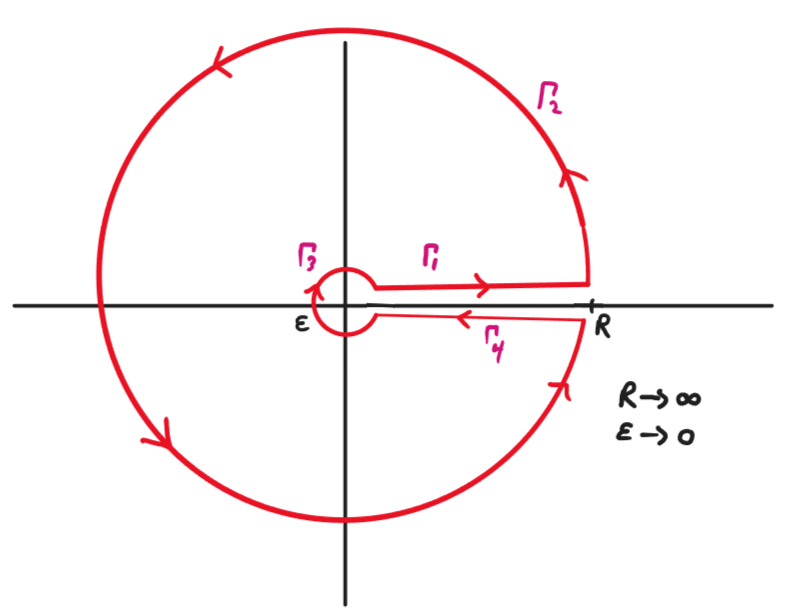
\includegraphics[width=0.6\textwidth]{Images/ComplexAnalysisPictures/KeyHole.png}}
Ex:
\begin{align*}
    &\int_0^\infty\frac{x^{\frac{1}{3}}}{x^2+1}dx\\
    &f(z)=\frac{z^\frac{1}{3}}{z^2+1}\\
    &I=\int_{\Gamma_1}\frac{z^{\frac{1}{3}}}{z^2+1}dz\\
    &z=\pm i\\
    &Q(z)=z^2+1\Ra Q'(z)=2z\Ra Q'(\pm i)=\pm 2i\\
    &P(i)=(i)^{\frac{1}{3}}= e^{i\frac{\pi}{6}}\\
    &P(-i)=\brround{e^{i\frac{3\pi}{2}}}^{\frac{1}{3}}=e^{i\frac{\pi}{2}}\\
    &\Res\brround{\frac{z^{\frac{1}{3}}}{z^2+1};i}=\frac{e^{i\frac{\pi}{6}}}{2i}\\
    &\Res\brround{\frac{z^{\frac{1}{3}}}{z^2+1};-i}=-\frac{e^{i\frac{\pi}{2}}}{2i}\\
    &\Gamma_4:\ |z|=\epsilon\\
    &\brvertical{\int_{\Gamma_4}\frac{z^{\frac{1}{3}}}{z^2+1}dz}\leq \max_{|z|=\epsilon}\brvertical{\frac{z^{\frac{1}{3}}}{z^2+1}}2\pi \epsilon=\frac{2\pi\epsilon^{\frac{4}{3}}}{1-\epsilon^2}\to0\\\
    &\Gamma_2:\ |z|=R\\
    &\brvertical{\int_{\Gamma_2}\frac{z^{\frac{1}{3}}}{z^2+1}dz}\leq\max_{|z|=R}\brvertical{\frac{z^{\frac{1}{3}}}{z^2+1}}2\pi R=\frac{2\pi R^{\frac{4}{3}}}{R^2-1}\to 0\\
    &\Gamma_1:\ z=r,\ 0<r<\infty\\
    &\Gamma_3:\ z=re^{2\pi i}\\
    &\int_{\Gamma_1}\frac{z^{\frac{1}{3}}}{z^2+1}dz+\int_{\Gamma_3}\frac{z^{\frac{1}{3}}}{z^2+1}dz=\brround{1-e^{i\frac{2\pi}{3}}}I=2\pi i\brround{\frac{e^{i\frac{\pi}{6}}}{2i}-\frac{e^{i\frac{\pi}{2}}}{2i}}\\
    &\brround{e^{-i\frac{\pi}{3}}-e^{i\frac{\pi}{3}}}I=\pi\brround{e^{-i\frac{\pi}{6}}-e^{i\frac{\pi}{6}}}\Ra \sin\bfrac{\pi}{3}I=\pi\sin\bfrac{\pi}{6}\\
    &I=\frac{\pi\bfrac{1}{2}}{\bfrac{\sqrt{3}}{2}}=\frac{\pi}{\sqrt{3}}
\end{align*}
\textit{Type VII:}\\
If we have an integral of the form
\[\int_0^{\infty}\frac{P(x)}{Q(x)}\ln xdx\]
then we can use the key-hole contour to solve the integral.\\
\centerline{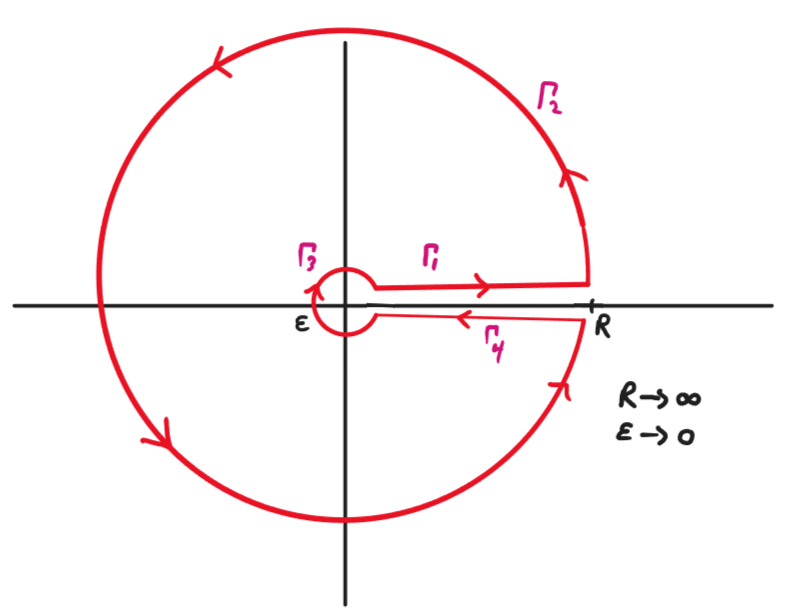
\includegraphics[width=0.6\textwidth]{Images/ComplexAnalysisPictures/KeyHole.png}}
Ex:
\begin{align*}
    &\int_0^\infty\frac{\ln x}{x^2+4}dx\\
    &f(z)=\frac{\log^2 z}{z^2+4}=\frac{\brround{\ln r+i\varphi}^2}{z^2+4},\ \varphi\in\brround{0,2\pi}\\
    &z=\pm 2i\\
    &Q(z)=z^2+4\Ra Q'(z)=2z\Ra Q'(\pm 2i)=\pm 4i\\
    &P(z)=\ln^2r+2i\ln (r)\varphi-\varphi^2\\
    &P(2i)=\ln^2 2+\pi i\ln 2-\frac{\pi^2}{4}\\
    &P(-2i)=\ln^2 2+3\pi i\ln 2-\frac{9\pi^2}{4}\\
    &\Res\brround{f(z);2i}=\frac{\ln^2 2+\pi i\ln 2-\frac{\pi^2}{4}}{4i}\\
    &\Res\brround{f(z);-2i}=-\frac{\ln^2 2+3\pi i\ln 2-\frac{9\pi^2}{4}}{4i}\\
    &\Gamma_1:\ z=r\\
    &\int_{\Gamma_1}f(z)dz=\int_\epsilon^R\frac{\ln^2r}{r^2+4}dz\\
    &\Gamma_3:\ z=re^{2\pi i}\\
    &\int_{\Gamma_3}f(z)dz=-\int_\epsilon^R\frac{\ln^2r+4\pi i\ln r-4\pi^2}{r^2+4}dr\\
    &\Gamma_2:\ z=Re^{i t}\\
    &\brvertical{\int_{\Gamma_2}f(z)dz}\leq\max_{|z|=R}\brvertical{\frac{\ln^2R+2i t\ln R-t^2}{z^2+4}}2\pi R=\max_{0<t<2\pi}\frac{2\pi R\sqrt{(\ln^2R-t^2)^2+4t^2\ln^2R}}{R^2-4}\to0\\
    &\Gamma_4:\ z=\epsilon e^{it}\\
    &\brvertical{\int_{\Gamma_4}f(z)dz}\leq\max_{|z|=\epsilon}\brvertical{\frac{\ln^2\epsilon+2i t\ln \epsilon-t^2}{z^2+4}}2\pi \epsilon=\max_{0<t<2\pi}\frac{2\pi \epsilon\sqrt{(\ln^2\epsilon-t^2)^2+4t^2\ln^2\epsilon}}{4-\epsilon^2}\to0\\
    &\int_0^\infty\frac{\ln^2 r}{r^2+4}dr-\int_0^\infty\frac{(\ln r+i2\pi)^2}{r^2+4}dr=2\pi i\brround{\frac{-2\pi i\ln 2+\frac{8\pi^2}{4}}{4i}}\\
    &-4\pi i\int_0^\infty\frac{\ln r}{r^2+4}dr=\frac{\pi}{2}\brround{-2\pi i\ln2+\frac{8\pi^2}{4}}\\
    &\Im\brround{4\pi i\int_0^\infty\frac{\ln r}{r^2+4}dr}=\pi^2\ln 2\\
    &4\pi I=\pi^2\ln 2\\
    &I=\frac{\pi\ln2}{4}
\end{align*}
We can combine a lot of these tricks and techniques to solve more complicated integrals.\\
Ex:
\begin{align*}
    &\int_0^\infty\frac{\sqrt{x}\ln x}{x^2+1}dx
\end{align*}
\centerline{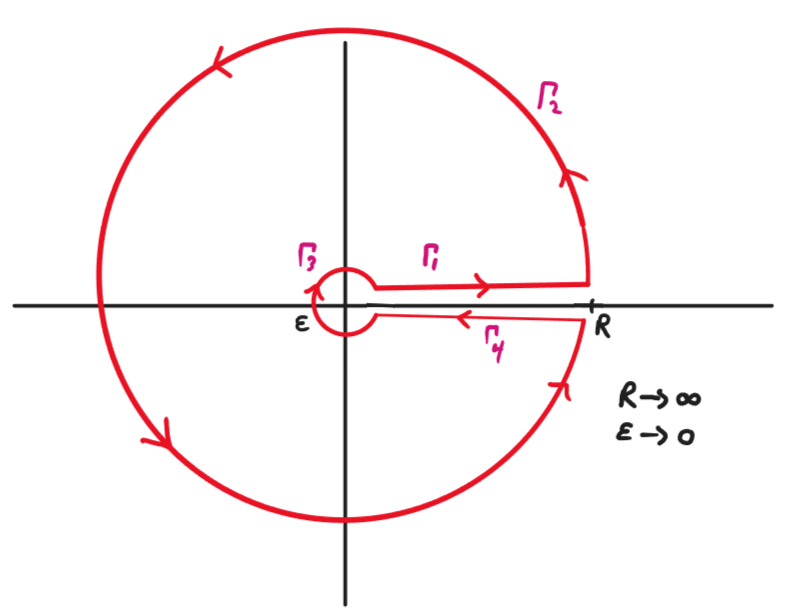
\includegraphics[width=0.6\textwidth]{Images/ComplexAnalysisPictures/KeyHole.png}}
\begin{align*}
    &f(z)=\frac{z^\frac{1}{2}\log z}{z^2+1}=\frac{\sqrt{r}e^{i\frac{\varphi}{2}}(\ln r+i\varphi)}{z^2+1},\ \varphi\in(0,2\pi)\\
    &\int_{\Gamma_1}\frac{\sqrt{r}e^{i\frac{\varphi}{2}}(\ln r+i\varphi)}{z^2+1}dz\\
    &z=\pm i\\
    &Q(z)=z^2+1\Ra Q'(z)=2z\Ra Q'(\pm i)=\pm 2i\\
    &P(z)=\sqrt{r}e^{i\frac{\varphi}{2}}\brround{\ln r+i\varphi}\\
    &P(i)=e^{i\frac{\pi}{4}}\brround{i\frac{\pi}{2}}\\
    &P(-i)=e^{i\frac{3\pi}{4}}\brround{i\frac{3\pi}{2}}\\
    &\Res\brround{f(z);i}=\frac{\pi e^{i\frac{\pi}{4}}}{4}\\
    &\Res\brround{f(z);-i}=-\frac{3\pi e^{i\frac{3\pi}{4}}}{4}\\
    &\int_0^\infty\frac{\sqrt{r}\ln r}{r^2+1}dr-\int_0^\infty\frac{\sqrt{r}(-1)(\ln r+2\pi i)}{r^2+1}dr=2\pi i\brround{\frac{\pi e^{i\frac{\pi}{4}}}{4}-\frac{3\pi e^{i\frac{3\pi}{4}}}{4}}\\
    &\Gamma_1:\ z=r\\
    &\int_{\Gamma_1}f(z)dz=\int_\epsilon^R\frac{\sqrt{r}\ln r}{r^2+1}dr\\
    &\Gamma_3:\ z=re^{2\pi i}\\
    &\int_{\Gamma_3}f(z)dz=-\int_\epsilon^R\frac{\sqrt{r}(-1)(\ln r+2\pi i)}{r^2+1}dr\\
    &\Gamma_2:\ z=Re^{it}\\
    &\brvertical{\int_{\Gamma_2}f(z)dz}\leq\max_{|z|=R}\brvertical{\frac{\sqrt{R}e^{i\frac{t}{2}}\brround{\ln R+i t}}{z^2+1}}2\pi R=\max_{0< t<2\pi}\frac{2\pi R^\frac{3}{2}\sqrt{\ln^2R+t^2}}{R^2-1}\to0\\
    &\Gamma_4:\ z=\epsilon e^{it}\\
    &\brvertical{\int_{\Gamma_4}f(z)dz}\leq\max_{|z|=\epsilon}\brvertical{\frac{\sqrt{\epsilon}e^{i\frac{t}{2}}\brround{\ln \epsilon+i t}}{z^2+1}}2\pi \epsilon=\max_{0< t<2\pi}\frac{2\pi \epsilon^\frac{3}{2}\sqrt{\ln^2\epsilon+t^2}}{1-\epsilon^2}\to0\\
    &2\int_0^\infty\frac{\sqrt{r}\ln r}{r^2+1}dr+2\pi i\int_0^\infty\frac{\sqrt{r}}{r^2+1}dr=\frac{\pi^2 i}{2}\brround{e^{i\frac{\pi}{4}}-3e^{i\frac{3\pi}{4}}}=\frac{\pi^2 i}{2}\brround{\frac{1}{\sqrt{2}}+\frac{i}{\sqrt{2}}+\frac{3}{\sqrt{2}}-\frac{3i}{\sqrt{2}}}\\
    &2\int_0^\infty\frac{\sqrt{r}\ln r}{r^2+1}dr=\Re\brround{\frac{\pi^2 i}{2}\brround{\frac{4}{\sqrt{2}}-\frac{2i}{\sqrt{2}}}}=\frac{\pi^2}{\sqrt{2}}\\
    &I=\frac{\pi^2}{2\sqrt{2}}
\end{align*}
Ex2:
\begin{align*}
    &\int_0^\infty\frac{\ln x}{x^3+1}dx
\end{align*}
\centerline{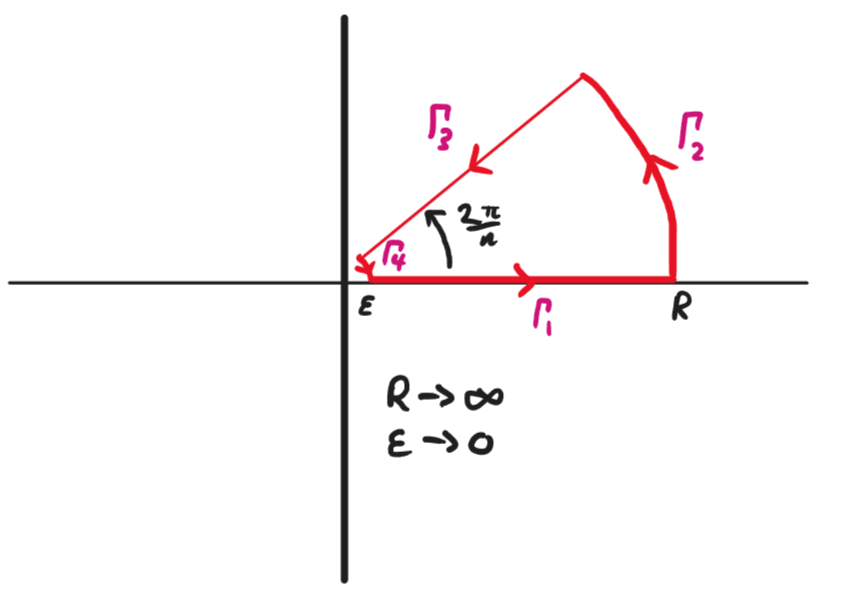
\includegraphics[width=0.6\textwidth]{Images/ComplexAnalysisPictures/Pizza.png}}
\begin{align*}
    &f(z)=\frac{\log z}{z^3+1}\\
    &\Gamma_1:\ z=r\\
    &\int_{\Gamma_1}f(z)dz=\int_\epsilon^R\frac{\ln r}{r^3+1}dr\\
    &\Gamma_3:\ z=re^{i\frac{2\pi}{3}}\\
    &\int_{\Gamma_3}f(z)dz=-e^{i\frac{2\pi}{3}}\int_\epsilon^R\frac{\ln r+i\frac{2\pi}{3}}{r^3+1}dr\\
    &\Gamma_2:\ z=Re^{i t}\\
    &\brvertical{\int_{\Gamma_2}f(z)dz}=\brvertical{\int_{\Gamma_2}\frac{\log z}{z^3+1}dz}\leq\max_{|z|=R}\brvertical{\frac{\log z}{z^3+1}}\frac{2\pi R}{3}=\max_{0< t< \frac{2\pi}{3}}\frac{\sqrt{\ln^2R+t^2}}{R^3-1}\frac{2\pi R}{3}\to 0\\
    &\Gamma_4:\ z=\epsilon e^{it}\\
    &\brvertical{\int_{\Gamma_2}f(z)dz}=\brvertical{\int_{\Gamma_2}\frac{\log z}{z^3+1}dz}\leq\max_{|z|=\epsilon}\brvertical{\frac{\log z}{z^3+1}}\frac{2\pi \epsilon}{3}=\max_{0< t< \frac{2\pi}{3}}\frac{\sqrt{\ln^2\epsilon+t^2}}{1-\epsilon^3}\frac{2\pi \epsilon}{3}\to 0\\
    &z^3+1=0\Ra z=(-1)^\frac{1}{3}=(e^{i\pi+2\pi ki})^\frac{1}{3}=e^{i\frac{\pi}{3}+i\frac{2\pi k}{3}}\\
    &Q(z)=z^3+1\Ra Q'(z)=3z^2\Ra Q'(e^{i\frac{\pi}{3}})=3e^{i\frac{2\pi}{3}}\\
    &P(z)=\log z\Ra P(e^{i\frac{\pi}{3}})=i\frac{\pi}{3}\\
    &\Res\brround{f(z);e^{i\frac{\pi}{3}}}=\frac{\pi i}{9e^{i\frac{2\pi}{3}}}\\
    &\int_0^\infty\frac{\ln r}{r^3+1}dr-e^{i\frac{2\pi}{3}}\int_0^\infty\frac{\ln r+i\frac{2\pi}{3}}{r^3+1}dr=2\pi i\Res\brround{f(z);e^{i\frac{\pi}{3}}}\\
    &\brround{1-e^{i\frac{2\pi}{3}}}I-\frac{2\pi i}{3}e^{i\frac{2\pi}{3}}\int_0^\infty\frac{dr}{r^3+1}=2\pi i\frac{\pi i}{9e^{i\frac{2\pi}{3}}}=-\frac{2\pi^2}{9}e^{-i\frac{2\pi}{3}}\\
    &\brround{e^{-i\frac{2\pi}{3}}-1}I-\frac{2\pi i}{3}\int_0^\infty\frac{dr}{r^3+1}=-\frac{2\pi^2}{9}e^{-i\frac{4\pi i}{3}}\\
    &\Re\brround{e^{-i\frac{2\pi}{3}}-1}I=-\frac{2\pi^2}{9}\Re\brround{e^{-i\frac{4\pi}{3}}}\\
    &\brround{\cos\bfrac{2\pi}{3}-1}I=-\frac{2\pi^2}{9}\cos\bfrac{4\pi}{3}\\
    &I=-\frac{2\pi^2\brround{-\frac{1}{2}}}{9\brround{-\frac{1}{2}-1}}=-\frac{\pi^2}{9\bfrac{3}{2}}\\
    &I=-\frac{2\pi^2}{27}
\end{align*}
Ex3:
\begin{align*}
    &\int_0^\infty\frac{dx}{(x+1)(x^2+2x+5)}
\end{align*}
\centerline{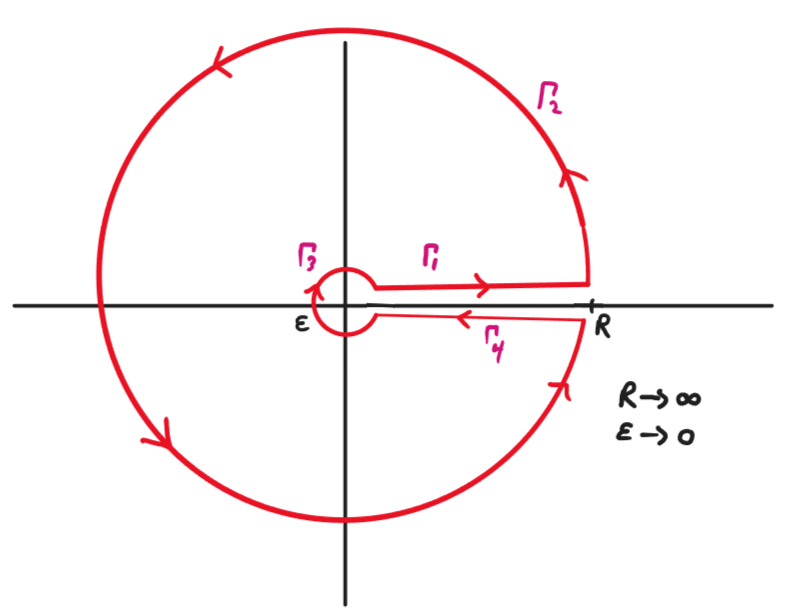
\includegraphics[width=0.6\textwidth]{Images/ComplexAnalysisPictures/KeyHole.png}}
\begin{align*}
    &f(z)=\frac{\log z}{(z+1)(z^2+2z+5)}\\
    &z=-1\\
    &z=\frac{-2\pm\sqrt{4-20}}{2}=-1\pm 2i\\
    &Q(z)=(z+1)(z^2+2z+5)\Ra Q'(z)=(z+1)(2z+2)+z^2+2z+5=2(z+1)^2+z^2+2z+5\\
    &Q'(-1)=1-2+5=4\\
    &Q'(-1\pm 2i)=2(\pm 2i)^2=-8\\
    &P(z)=\log z\\
    &P(-1)=\pi i\\
    &P(-1\pm 2i)=\ln\sqrt{5}+i\varphi_{1,2}\\
    &\Res\brround{f(z);-1}=\frac{\pi i}{4}\\
    &\Res\brround{f(z);-1\pm 2i}=-\frac{\ln\sqrt{5}+i\varphi_{1,2}}{8}\\
    &\varphi_1+\varphi_2=2\pi\\
    &\Res\brround{f(z);-1+2i}+\Res\brround{f(z)-1-2i}=-\frac{2\ln\sqrt{5}-2\pi i}{8}\\
    &\Gamma_1:\ z=r\\
    &\int_{\Gamma_1}f(z)=\int_\epsilon^R\frac{\ln r}{(r+1)(r^2+2r+5)}dr\\
    &\Gamma_3:\ z=re^{2\pi i}\\
    &\int_{\Gamma_3}f(z)dz=-\int_\epsilon^R\frac{\ln r+2\pi i}{(r+1)(r^2+2r+5)}dr\\
    &\Gamma_2:\ z=Re^{it}\\
    &\brvertical{\int_{\Gamma_2}f(z)dz}\leq\max_{|z|=R}\brvertical{\frac{\log z}{(z+1)(z^2+2z+5)}}2\pi R\leq\max_{0<t<2\pi}\frac{2\pi R\sqrt{\ln^2R+t^2}}{(R-1)(R^2-2R-5)}\to 0\\
    &\Gamma_4:\ z=\epsilon e^{it}\\
    &\brvertical{\int_{\Gamma_4}f(z)dz}\leq\max_{|z|=\epsilon}\brvertical{\frac{\log z}{(z+1)(z^2+2z+5)}}2\pi \epsilon\leq\max_{0<t<2\pi}\frac{2\pi \epsilon\sqrt{\ln^2\epsilon+t^2}}{(1-\epsilon)(5-2\epsilon-\epsilon^2)}\to 0\\
    &\int_0^\infty\frac{\ln r}{(r+1)(r^2+2r+5)}dr-\int_0^\infty\frac{\ln r+2\pi i}{(r+1)(r^2+2r+5)}dr=2\pi i\sum_{j=1}^3\Res\brround{f(z);z_j}\\
    &-2\pi i\int_0^\infty\frac{dr}{(r+1)(r^2+2r+5)}=2\pi i\brround{\frac{\pi i}{4}-\frac{2\ln\sqrt{5}-2\pi i}{8}}\\
    &I=-\frac{2\pi i}{8}+\frac{\ln 5-2\pi i}{8}\\
    &I=\frac{\ln 5}{8}
\end{align*}

\subsubsection{Fourier Transforms}
We define the Fourier Transform of a function $f(x)$ as
\[\hat{f}(k)=\int_{-\infty}^\infty e^{-ikx}f(x)dx\]
Ex: $f(x)=\frac{1}{1+x^2}$
\begin{align*}
    &\hat{f}(k)=\int_{-\infty}^\infty\frac{e^{-ikx}}{1+x^2}dx=\pi e^{-|k|}
\end{align*}
The inverse Fourier Transform is defined as
\[f(x)=\frac{1}{2\pi}\int_{-\infty}^\infty e^{ikx}\hat{f}(k)dk\]
Two key properties of the Fourier Transform are
\begin{itemize}
    \item Derivatives
    \[\mathcal{F}\brcurly{f'(x)}=-ik\hat{f}(k),\quad \mathcal{F}\brcurly{f''(x)}=(-ik)^2\hat{f}(k)\]
    \item Convolution
    \[\mathcal{F}\brcurly{f * g}=\hat{f}(k)\hat{g}(k)\]
    \[f * g(x)=\int_{-\infty}^\infty f(x-y)g(y)dy\]
\end{itemize}
Ex: Find the general solution to the ODE
\begin{align*}
    &u''''+u=g(x)\\
    &(k^4+1)\hat{u}=\hat{g}(k)\\
    &\hat{u}=\frac{\hat{g}(k)}{k^4+1}=\hat{f}(k)\hat{g}(k)\\
    &u(x)=f(x)*g(x)=\F^{-1}\brcurly{\frac{1}{k^4+1}}*g(x)\\
    &f(x)=\frac{1}{2\pi}\int_{-\infty}^\infty\frac{1}{k^4+1}e^{ikx}dk\\
    &k^4+1=0\Ra k=e^{i\frac{\pi}{4}+ik\frac{\pi}{2}}
\end{align*}
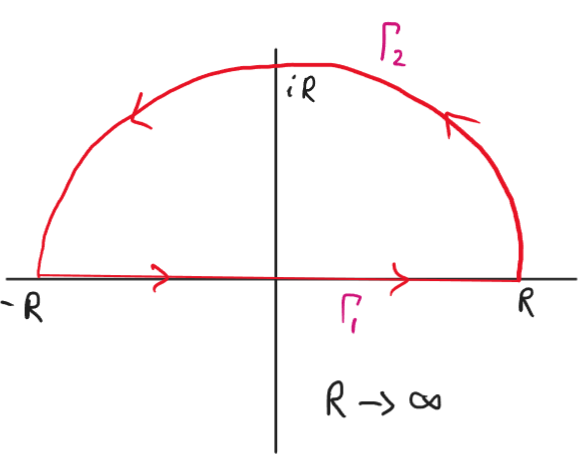
\includegraphics[scale=0.6]{Images/ComplexAnalysisPictures/HalfMoon.png}
\begin{align*}
    &\Gamma_1:\ z=r\\
    &\int_{\Gamma_1}\frac{e^{ikx}}{k^4+1}dk=\int_{-\infty}^\infty\frac{e^{ikx}}{k^4+1}dk\\
    &\Gamma_2:\ k=Re^{i t},\ 0\leq t\leq \pi\\
    &\brvertical{\int_{\Gamma_2}\frac{e^{ikx}}{k^4+1}dk}\leq\max_{|k|=R}\brvertical{\frac{e^{ikx}}{k^4+1}}\pi R=\max_{0\leq t\leq \pi}\frac{\pi Re^{-R\sin t}}{R^4-1}=\frac{\pi R}{R^4-1}\to 0\\
    &Q(k)=k^4+1\Ra Q'(k)=4k^3\\
    &Q'(e^{i\frac{\pi}{4}})=4e^{i\frac{3\pi}{4}}\\
    &Q'(e^{i\frac{3\pi}{4}})=4e^{i\frac{9\pi}{4}}=4e^{i\frac{\pi}{4}}\\
    &P\brround{\frac{1}{\sqrt{2}}+\frac{i}{\sqrt{2}}}=e^{-\frac{x}{\sqrt{2}}}e^{i\frac{x}{\sqrt{2}}}\\
    &P\brround{-\frac{1}{\sqrt{2}}+\frac{i}{\sqrt{2}}}=e^{-\frac{x}{\sqrt{2}}}e^{-i\frac{x}{\sqrt{2}}}\\
    &\Res\brround{\frac{e^{ikx}}{k^4+1};e^{i\frac{\pi}{4}}}=\frac{e^{-\frac{x}{\sqrt{2}}}e^{i\frac{x}{\sqrt{2}}}}{4e^{i\frac{3\pi}{4}}}\\
    &\Res\brround{\frac{e^{ikx}}{k^4+1};e^{i\frac{\pi}{4}}}=\frac{e^{-\frac{x}{\sqrt{2}}}e^{-i\frac{x}{\sqrt{2}}}}{4e^{i\frac{\pi}{4}}}\\
    &I=2\pi i\frac{e^{-\frac{x}{\sqrt{2}}}}{4}\brround{e^{i\frac{x}{\sqrt{2}}}e^{-i\frac{3\pi}{2}}+e^{-i\frac{x}{\sqrt{2}}}e^{-i\frac{\pi}{4}}}=\frac{\pi i}{2}e^{-\frac{x}{\sqrt{2}}}e^{-i\frac{\pi}{2}}\brround{e^{i\frac{x}{\sqrt{2}}}e^{-i\frac{\pi}{4}}+e^{-i\frac{x}{\sqrt{2}}}e^{i\frac{\pi}{4}}}\\
    &I=\frac{\pi}{2}e^{-\frac{x}{\sqrt{2}}}\brround{\frac{e^{i\frac{x}{\sqrt{2}}}}{\sqrt{2}}(1-i)+\frac{e^{-i\frac{x}{\sqrt{2}}}}{\sqrt{2}}(1+i)}=\frac{\pi}{\sqrt{2}}e^{-\frac{x}{\sqrt{2}}}\brround{\frac{e^{i\frac{x}{\sqrt{2}}}+e^{-i\frac{x}{\sqrt{2}}}}{2}+\frac{e^{i\frac{x}{\sqrt{2}}}-e^{-i\frac{x}{\sqrt{2}}}}{2i}}\\
    &I=\frac{\pi}{\sqrt{2}}e^{-\frac{x}{\sqrt{2}}}\brround{\sin\bfrac{x}{\sqrt{2}}+\cos\bfrac{x}{\sqrt{2}}},\ x>0\\
    &\Ra f(x)=\frac{e^{-\frac{|x|}{\sqrt{2}}}}{2\sqrt{2}}\brround{\sin\bfrac{|x|}{\sqrt{2}}+\cos\bfrac{|x|}{\sqrt{2}}}\\
    &u_p(x)=\int_{-\infty}^\infty \frac{e^{-\frac{|x-y|}{\sqrt{2}}}}{2\sqrt{2}}\brround{\sin\bfrac{|x-y|}{\sqrt{2}}+\cos\bfrac{|x-y|}{\sqrt{2}}}g(y)dy\\
    &u_c(x)=c_1e^{\frac{1}{\sqrt{2}}(1+i)x}+c_2e^{\frac{1}{\sqrt{2}}(-1+i)x}+c_3e^{\frac{1}{\sqrt{2}}(-1-i)x}+c_4e^{\frac{1}{\sqrt{2}}(1-i)x}\\
    &\lim_{|x|\to\infty} u(x)=0\Ra u_c(x)=0\\
    &u(x)=\int_{-\infty}^\infty \frac{e^{-\frac{|x-y|}{\sqrt{2}}}}{2\sqrt{2}}\brround{\sin\bfrac{|x-y|}{\sqrt{2}}+\cos\bfrac{|x-y|}{\sqrt{2}}}g(y)dy
\end{align*}
Ex2: Find the general solution to the ODE
\begin{align*}
    &u''''-4u''+4u=g(x)\\
    &(k^4+4k^2+4)\hat{u}=\hat{g}(k)\\
    &\hat{u}=\frac{\hat{g}(k)}{k^4+4k^2+4}=\hat{f}(k)\hat{g}(k)\\
    &u(x)=f(x)*g(x)=\F^{-1}\brcurly{\frac{1}{k^4+4k^2+4}}*g(x)\\
    &f(x)=\frac{1}{2\pi}\int_{-\infty}^\infty\frac{e^{ikx}}{k^4+4k^2+4}dk\\
    &k^4+4k^2+4=0\Ra (k^2+2)^2=0\Ra k^2=-2\Ra k=\pm \sqrt{2}i\\
    &h(k)=\frac{e^{ikx}}{(k+\sqrt{2}i)^2(k-\sqrt{2}i)^2}\\
    &h_\pm(k)=\frac{e^{ikx}}{(k\pm \sqrt{2}i)^2}\\
    &h_\pm'(k)=\frac{ixe^{ikx}}{(k\pm \sqrt{2}i)^2}-\frac{2e^{ikx}}{(k\pm \sqrt{2}i)^3}\\
    &h_\pm'(\pm \sqrt{2}i)=\frac{ixe^{\mp \sqrt{2}x}}{-8}-\frac{2e^{\mp 2x}}{\mp16\sqrt{2}i}=\frac{e^{\mp \sqrt{2}x}}{8}\brround{-ix\pm \frac{1}{\sqrt{2}i}}=\frac{ie^{\mp\sqrt{2}x}}{8}\brround{-x\mp\frac{1}{\sqrt{2}}}
\end{align*}
The contour is the same as in Ex1 and the integral is equal to the sum of the residues in $\Im(k)>0$
\begin{align*}
    &I=2\pi i\Res\brround{\frac{e^{ikx}}{k^4+4k^2+4};2i}\\
    &I=2\pi i\frac{i}{8}\brround{-x-\frac{1}{\sqrt{2}}}e^{-\sqrt{2}x}\\
    &I=\frac{\pi}{8}(2x+\sqrt{2})e^{-\sqrt{2}x}\\
    &f(x)=\frac{1}{16}\brround{2|x|+\sqrt{2}}e^{-\sqrt{2}|x|}\\
    &u_p(x)=f(x)*g(x)=\frac{1}{16}\int_{-\infty}^\infty\brround{2|x-y|+\sqrt{2}}e^{-\sqrt{2}|x-y|}g(y)dy\\
    &u_c(x)=c_1e^{\sqrt{2}ix}+c_2e^{-\sqrt{2}ix}\\
    &\lim_{|x|\to\infty} u(x)=0\Ra u_c(x)=0\\
    &u(x)=\frac{1}{16}\int_{-\infty}^\infty\brround{2|x-y|+\sqrt{2}}e^{-\sqrt{2}|x-y|}g(y)dy
\end{align*}
In general, when given an ODE of the form $y^{(n)}+\cdots+a_ny=g$ then we can take the Fourier trasnform of both sides to get
\[p(-ik)\hat{y}=\hat{g}\]
Then we can rearrange to solve for $\hat{y}$
\[\hat{y}=\frac{1}{p(-ik)}\hat{g}\]
Then define $\hat{f}=\frac{1}{p(-ik)}$ and use the convolution property $y=f * g$
\subsubsection{Laplace Transforms}
The Laplace Transform of a function $f(t)$ is defined as
\[\hat{f}(s)=\lap[f](s)=\int_0^\infty f(t)e^{-st}dt\]
We can define the inverse Laplace transform using Melin's Formula
\[f(t)=\frac{1}{2\pi i}\int_{\gamma-i\infty}^{\gamma+i\infty}\brround{\lap[f](z)e^{zt}}dz\]
We define $\gamma$ to be large enough such that all poles of $\lap[f](z)$ lie in $\Re(z)<\gamma$.
And so we can use the Cauchy Residue Theorem to solve the integral.
\[f(t)=\frac{1}{2\pi i}\int_{\gamma-i\infty}^{\gamma+i\infty}\brround{\lap[f](z)e^{zt}}dz=\sum_{j=1}^N\Res\brround{\lap[f](z)e^{zt};z_j}\]
Ex: Suppose $\lap[f](s)=\frac{1}{(s+1)^2(s+2)}$. Find the inverse Laplace transform, $f(t)$.
\begin{align*}
    &f(t)=\frac{1}{2\pi i}\int_{\gamma-i\infty}^{\gamma+i\infty}\brround{\frac{e^{zt}}{(z+1)^2(z+2)}}dz,\ \gamma>0\\
    &f(t)=\sum_{j=1}^2\Res\brround{\frac{e^{zt}}{(z+1)^2(z+2)};z_j}\\
    &f(t)=\Res\brround{\frac{e^{zt}}{(z+1)^2(z+2)};-1}+\Res\brround{\frac{e^{zt}}{(z+1)^2(z+2)};-2}\\
    &f(t)=\ddx{z}\bfrac{e^{zt}}{z+2}\eval_{z=-1}+\frac{e^{zt}}{(z+1)^2}\eval_{z=-2}=te^{-t}-e^{-t}+e^{-2t}
\end{align*}